
\documentclass[12pt,a4paper]{article}

\usepackage[utf8]{inputenc}
\usepackage{lmodern}
\usepackage[T1]{fontenc}
% paysage
% \usepackage[landscape]{geometry}
\usepackage{lscape}
\usepackage{graphicx}
% \graphicspath{ {images/} }

% headers footers
\usepackage{fancyhdr}
\pagestyle{fancy}

% référencer la dernière page
\usepackage{lastpage}

% pdf
\usepackage{pdfpages}

% math
\usepackage{amssymb}

\usepackage{multicol}
\usepackage{url}

\usepackage{multido}
\usepackage[utf8]{inputenc}
% \usepackage{lmodern}
\usepackage[T1]{fontenc}

\usepackage[sfdefault]{AlegreyaSans} %% Option 'black' gives heavier bold face
%% The 'sfdefault' option to make the base font sans serif
% \renewcommand*\oldstylenums[1]{{\AlegreyaSansOsF #1}}


\usepackage{multicol}

% \usepackage{pstricks,pst-plot,pst-node}
% \usepackage{pstricks-add}
\usepackage{pst-circ}
\usepackage{pst-magneticfield}
\usepackage{pst-electricfield}
\usepackage{graphicx}
\usepackage{amsmath,amsfonts,amssymb}
\usepackage{titlesec} 
\usepackage{float}
\usepackage{textcomp}
\usepackage{amssymb}
\usepackage[toc,page]{appendix}
\usepackage{listings} 

\lstset{language=Matlab}
\usepackage{lipsum}
\usepackage{enumerate}


%Numerotation par section des équations
\usepackage{amsmath}

\usepackage{tabularx}
\usepackage{longtable}

%------------------------------inclue les références
% \usepackage[nottoc, notlof, notlot]{tocbibind}
%\usepackage{biblatex}
% \usepackage{csquotes}

%\usepackage{etoolbox}
% \patchcmd{\chapter}{\thispagestyle{plain}}{\thispagestyle{fancy}}{}{}
\title{
	\Huge\textsc{Excavator arm}
}
\author{Mohamed Thebti} 

\begin{document}
	% retrait de la première ligne d'un paragraphe
	\setlength{\parindent}{0mm}
	
	\fancyhead[R]{\slshape \leftmark}
	\fancyhead[L]{\slshape Excavator arm}
	%\fancyhead[LE,RO]{\slshape \rightmark}
	% \fancyhead[LO,RE]{\slshape \leftmark}
	
	% \fancyfoot[C]{Travail de Master}
	\fancyfoot[L]{\slshape Mohamed Thebti}
	\fancyfoot[C]{}
	\fancyfoot[R]{\thepage}
	
	\maketitle
	\newpage
	
	\tableofcontents
	
	\newpage
	
	
	
	\section{Introduction}
	
	The objective of this report is compute the pressure and power of a excavator arm. 
	
	% 
\includegraphics[scale=.2]{oxford-2021-01.jpg}
	
	\section{Hydraulic cylinder}
	
	\subsection{Definition}
	An hydraulic cylinder is a mechanical system (jack), which converts hydraulic pressure to force and movement.
	
	Its component are a cylinder, in which a piston can translate freely. This movement is initiated by controlling the pressure on both sides of the piston. 
	
	\subsection{Hydraulic system}
	The engine of the excavator drives an hydraulic pump, which push water into the hydraulic system at specified velocity and pressure. The dimensions of the hoses determine the pressure at any point of the circuit. This will be further detailed in chapter ???.
	
	\subsection{Piston movement}
	By setting the pressure on both side of the piston, the movement of the piston can be controlled. \\
	
	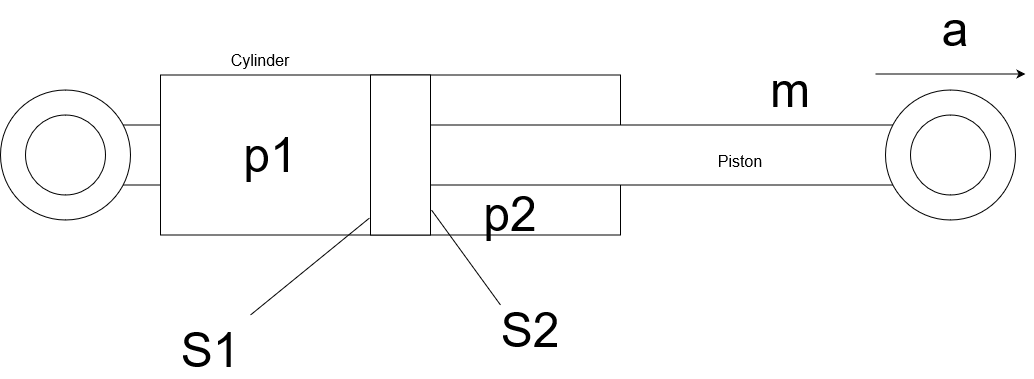
\includegraphics[scale=.35]{Hydraulic_cylinder.png}
	\\
	Second law of motion : 
	\begin{equation}
		\Sigma F = F_1 - F_2 = F_3 = p_1 \cdot S_1 - p_2 \cdot S_2= m \cdot a
	\end{equation}
	The difference of forces will cause an acceleration of the piston in one direction.
	$F_1$ and $F_2$ are the result of pressure $p_1$ $p_2$ on the area $S_1$ and $S_2$. \\
	
	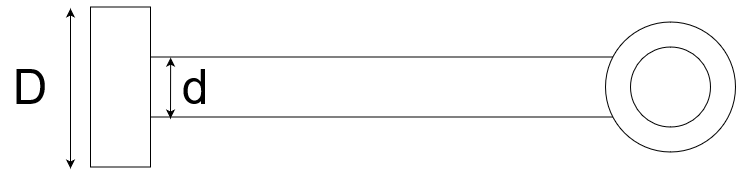
\includegraphics[scale=.35]{Hydraulic_cylinder_piston.png}
	\begin{equation}
		S_1 = \pi \cdot \frac{D^2}{4} = \pi \cdot R^2 
	\end{equation}
	\begin{equation}
		S_2 = \pi \cdot \frac{D^2}{4} - \pi \cdot \frac{d^2}{4} = \pi \cdot \frac{D^2-d^2}{4} = \pi (R^2-r^2)
	\end{equation}
	
	
	
	The acceleration is, by definition, the derivative of velocity:
	\begin{equation}
		a = \frac{dv}{dt}
	\end{equation}
	Integrating the acceleration once gives the velocity and twice the position. 
	\begin{equation}
		v = \int a \cdot dt = a \cdot t + v_0
	\end{equation}
	
	\begin{equation}
		x = \int \int a \cdot dt^2 = \frac{a}{2} \cdot t^2 + v_0 \cdot t + x_0
	\end{equation}
	
	\subsection{Arm movement}
	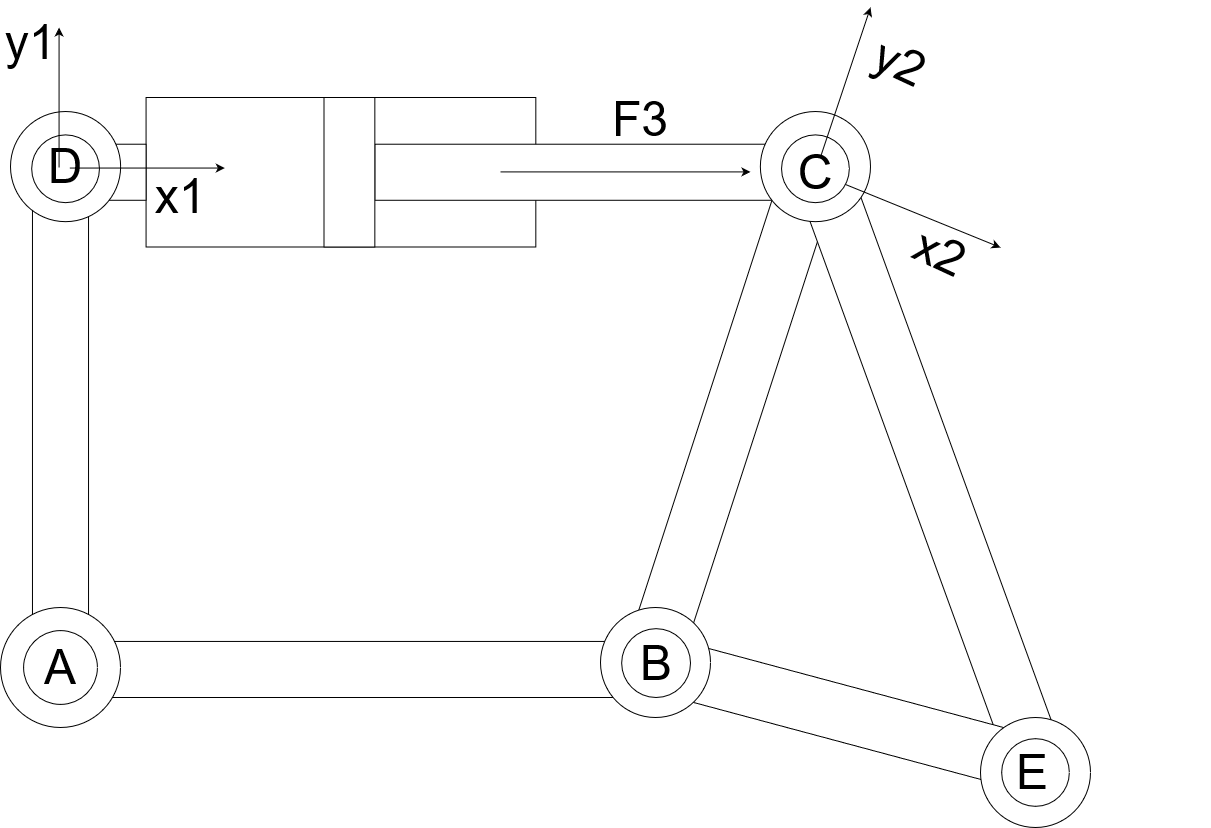
\includegraphics[scale=.35]{Quadrilatere.drawio.png}
	
	The triangle $BCE$ is the part of the excavator which needs to be controlled. Let's assure that it represents the bucket, situated at the extreme part of the arm. 
	
	The hydraulic cylinder applies a force $F_3$ on point C, making the triangle $BCE$ rotate on pivot $B$ with an angle $\beta$. 
	
	
	In chapter ???, we expose the Newton-Raphson method to determine angle $\beta$, between the segments $AB$ and $BC$.
	
	The torque equilibrium can be established in point $B$:
	\begin{equation}
		\sum T_B = I_{BCE} \cdot \alpha
	\end{equation}
	$\sum T_B$ : total torques applied on point $B$ in [Nm]\\
	$I_{BCE}$ : inertia of the bucket in $[kg m^2]$\\
	$\alpha$: angular acceleration in $[\frac{rad}{s^2}] $
	
	The sum of torques in point $B$ can be expressed as the vector/cross product of force verctor and position vertor. 
	\begin{equation}
		\sum \vec{T_B} = \sum \vec{F} \times \vec{d}
	\end{equation}
	The result is a vector that is perpendicular to both vectors : 
	$\vec{T_B} \perp \sum \vec{F}$ and 
	$\vec{T_B} \perp \vec{d}$.
	
	Let's assume that $F_3$ is the sum of the torques applied on the triangle $BCE$. In this case, the application point of $F_3$ is $C$. The scalar value of $\vec{T_B}$ is  the segment $\overline{BC}$ multiplied by the tangential force. This one is the projection of $F_3$ on $x_2$ axis, $F_3^{x_2}$:
	\begin{equation}
		T_B=||\vec{T_B}|| = F_3^{x_2} \cdot \overline{BC}
	\end{equation}
	The projection of $F_3$ on $x_2$ axis, $F_3^{y_2}$ is $\parallel$ to the segment $BC$. In this case, the vector/cross product is equal to $0$.
	Or : 
	\begin{equation}
		T_B=||\vec{T_B}|| = F_3 \cdot \overline{BF}
	\end{equation}
	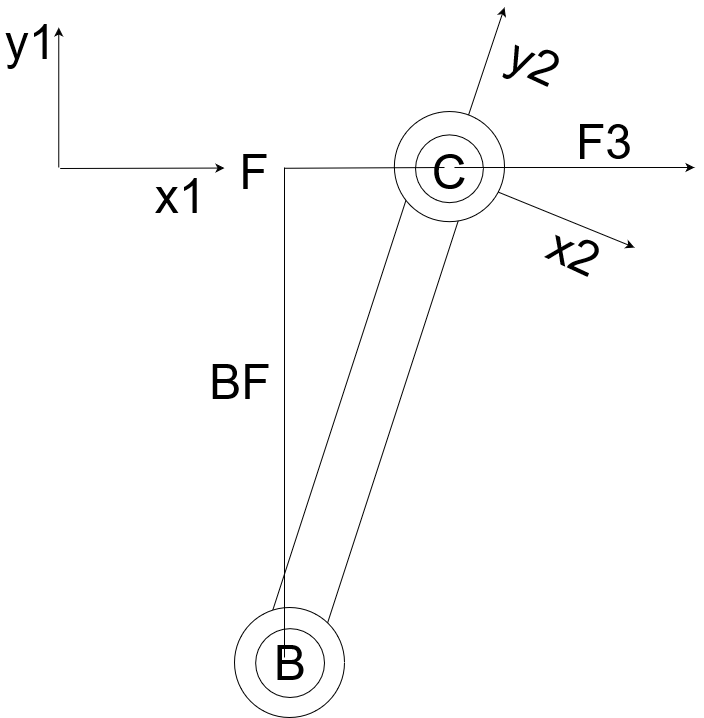
\includegraphics[scale=.35]{BCF.drawio.png}
	
	$\overline{B F}$ is the shortest distance between the force $F_3$ and point $B$.
	$\overline{B F}$ : projection of segment $\overline{BC}$ on axis $y_1$. 
	
	\begin{equation}
		\vec{BC}_{R_{1}}=
		\begin{bmatrix}
			\overline{BC}_{x_1} \\
			\overline{BC}_{y_1}\\
			0
		\end{bmatrix}_{R_{1}} 
	\end{equation}
	or : $F_3$ multiplied by $AD$, the distance between $F_3$ and $B$. (add schema with this 2 examples)
	
	Generally speaking, sum of Torque in B is 
	1. the sum of tangantial forces multiplied by
	2. easier : vector/cross product of a vector and distance vector to the $B$ point.  
	
	The Reynolds number is an non-dimensional number, and used to define if the fluid flow is laminar or turbulent. 
	
	\begin{equation}
		Re = \frac{\rho \cdot u \cdot L}{\mu}
	\end{equation}
	$\rho$ : density of the fluid\\
	$u$ : flow speed\\
	$L$ : characteristic linear dimension\\
	$\mu$ : dynamic viscosity of the fluid\\
	
	The characteristic linear dimension $L$ depends on the shape of the object of study. Here some example : 
	\begin{itemize}
		\item Plane wing : length of the wing
		\item Hydraulic pipe : diameter of the pipe
		\item Complex shape : the biggest dimension
	\end{itemize}
	Depending of the result, the flow can have 3 regimes
	
	\begin{itemize}
		\item If $Re$ <~ 2040, the flow is still considered laminar 
		\item If $Re$ >~ 2100, the flow is turbulent
		\item If 1800 <~ $Re$ <~ 2100, the flow is in the transition/intermediary range, which is a mix of laminar and turbulent \footnote{\url{https://en.wikipedia.org/wiki/Laminar_flow}}
	\end{itemize}
	
	For each regime, the drag force is different. 
	For turbulent and laminar regimes, the formula is as follows:
	\begin{equation}
		F_d^{turbulent} = \frac{1}{2} \cdot \rho \cdot C_D \cdot S \cdot u^2
	\end{equation}
	
	\begin{equation}
		F_d^{laminar} = C_F \cdot \rho \cdot  D^2 \cdot u^2\\
	\end{equation}
	$S$: cross frontal section\\
	$C_D$ : turbulent drag coefficient\\
	$C_F$ : laminar drag coefficient\\
	
	The intermediary regime is a mix from the 2 base regimes. In this situation, an approximation can be evaluated by computed the percent $Re$ compared to 1800 and 2100. 
	\begin{equation}
		F_d^{transition} = (1- \frac{Re - 1800}{2100-1800}) \cdot F_d^{laminar} + \frac{Re - 1800}{2100-1800} \cdot F_d^{turbulent}
	\end{equation}
	
	
	\newpage
	\section{Techniques}
	Prefabricated parts (PFP) /pre-manufactured parts (PMP)
	
	Instead of creating the same parts again and again, design the components and make them easily modifiable.
	for example, combine 2 parts to create a third one, which is useful in an other application. Then add them to the system in the assembly
	Example : threads : try the smallest possible size, for example M3 to M20. 
	
	Test them with small parts and check the tolerances. 
	The next step is to prepare small parts ready to be added to system parts. The final step is the merge the bodies. 
	
	
	table
	
	\begin{table}[ht]
		\caption{Holes and threaded holes} % title of Table
		\centering % used for centering table
		\begin{tabular}{c c c} % centered columns (4 columns)
			\hline\hline %inserts double horizontal lines
			Screw & Threaded hole diameter & Bore Hole (clearance) \\ [0.5ex] % inserts table
			%heading
			\hline % inserts single horizontal line
			M3 & 2.8 & 3.2 \\ % inserting body of the table
			4 & 35 & 144 \\
			5 & 45 & 300 \\ [1ex] % [1ex] adds vertical space
			\hline %inserts single line
		\end{tabular}\label{table:nonlin} % is used to refer this table in the text
	\end{table}
	
	Clearance
	To fix two part together, a clearance is needed.
	When two parts must be assembled together, a clearance of 0.1mm is enough. Then use the glue to fix the assembly. 
	
	
	
	\begin{table}[ht]
		\caption{Nonlinear Model Results} % title of Table
		\centering % used for centering table
		\begin{tabular}{c c c c} % centered columns (4 columns)
			\hline\hline %inserts double horizontal lines
			Case & Method\#1 & Method\#2 & Method\#3 \\ [0.5ex] % inserts table
			%heading
			\hline % inserts single horizontal line
			1 & 50 & 837 & 970 \\ % inserting body of the table
			2 & 47 & 877 & 230 \\
			3 & 31 & 25 & 415 \\
			4 & 35 & 144 & 2356 \\
			5 & 45 & 300 & 556 \\ [1ex] % [1ex] adds vertical space
			\hline %inserts single line
		\end{tabular}\label{table:nonlin} % is used to refer this table in the text
	\end{table}
	
	
	
	\begin{equation}
		Length_{lattitude}(\phi) = 111132.92-559.82 \cdot cos(2 \cdot \phi)+1.175*cos(4 \cdot \phi)-0.0023 \cdot cos(6 \cdot \phi)= ... [m/degree]
	\end{equation}
	1 degree longitude at latitude phi
	\begin{equation}
		Length_{longitude}(\phi) =
		111412.84-93.5 \cdot cos(3 \cdot \phi)+ 0.118 \cdot cos(5 \cdot \phi)= ... [m/degree]
	\end{equation}
	
	\newpage
	\section{Schéma cinématique}
	
	
	\subsection{Vecteurs positions}
	origine : centre de rotation verticale se trouvant sous les pâles principales.
	\medbreak
	position  des pâles principales ($pp$) : vecteur verticale
	\medbreak
	position de l'hélice arrière : 
	vecteur allant de l'origine vers l'hélice ($h$) arrière. 
	
	
	\newpage
	\section{Angular momentum}
	
	\subsection{Formula}
	\begin{equation}
		\vec{L}=\vec{OA} \otimes \vec{P}=\vec{r} \otimes \vec{P}=\vec{r} \otimes m \cdot \vec{v}=\vec{I} \otimes \vec{\omega}
	\end{equation}
	$\vec{L}$ : Angular Momentum [$kg \cdot \frac{m^2}{s}$]\\
	$\vec{OA}$ and $r$: position of the mass [$m$] according to a referance\\
	$\vec{P}$ : linear momentum [$kg\cdot \frac{m}{s}$]\footnote{$\vec{L}$ is perpendicular to both $\vec{P}$ and $\vec{r}$}\\
	$\vec{v}$ : velocity [$\frac{m}{s}$]
	$I$ : moment of inertia [$m^2 \cdot kg \cdot$]\\
	$\omega$ : angular speed [$\frac{rad}{s}$]
	
	Torque : 
	\begin{equation}
		M = \frac{d\vec{L}}{dt}=\frac{d(\vec{I} \otimes \vec{\omega})}{dt}
	\end{equation}
	\medbreak
	if we consider a particule of mass $m$, $\vec{r}$ is the position of the center of mass.
	If it is a solid object, $L$ is first computed according to the axis of rotation of the object : 
	\begin{equation}
		\vec{L}_{ar}=\vec{I}_{ar} \otimes \vec{\omega}_{ar}
	\end{equation}
	To compute the angular moment according to an other axis of rotation (new referance), we use the Huygens-Steiner theorem (or the Parallel axis theorem) : 
	\begin{equation}
		\vec{L}_{0}=\vec{I}_{0} \otimes \vec{\omega}_{cm}\\
	\end{equation}
	\begin{equation}
		\vec{I}_{0} = \vec{I}_{ar} + m\cdot d^2
	\end{equation}
	with $d$ the distance between the axis of rotation of the object and the new referance. 
	\subsection{Condition of stability}
	
	Main rotor(s):
	\begin{equation}
		\vec{L}_{mr}=\vec{r}_{mr} \otimes m_{mr} \cdot \vec{v_{mr}}=\vec{I_{mr}} \otimes \vec{\omega_{mr}}
	\end{equation}
	
	
	Rear rotor : 
	\begin{equation}
		\vec{L}_{rr}=\vec{r}_{rr} \otimes m_{rr} \cdot \vec{v_{rr}}=\vec{I_rr} \otimes \vec{\omega_{rr}}
	\end{equation}
	
	assurer la stabilité lors du vol: les moments cinétiques doivent s'annuler. (poser la formule et résoudre)
	\begin{equation}
		\vec{L_{mr}}=\vec{L_{rr}}
	\end{equation}
	
	or
	
	The generated torque is compensated : 
	\begin{equation}
		\sum \vec{M_{mr}}=\sum \vec{M_{rr}}
	\end{equation}
	
	find a relation between $\omega_{mr}$ and $\omega_{rr}$ -> determine the transmission ratio
	
	\subsection{Pivots à droite et à gauche}
	pour tourner à gauche ou doite, on ne doit plus satisfaire la condition de stabilité. le pilote utiliser le pédalier pour accélérer/ralentir l'hélice arrière. ainsi les moments cinétiques ne sont plus égaux.
	\medbreak
	calculer l'effet de rotation sur l'hélicoptère si l'hélice est accélérée/ralentie de 10,20,30,.. $\%$. mettre un tableau. calculer la vitesse de rotation dans ces cas-là. 
	
	
	\begin{equation}
		\begin{bmatrix}
			0 \\
			0\\
			l_1
		\end{bmatrix}_{R_{1}} \enspace
		\vec{AB}_{R_{2}}=
		\begin{bmatrix}
			0 \\
			l_2\\
			0
		\end{bmatrix}_{R_{2}} \enspace
		\vec{BC}_{R_{3}}=
		\begin{bmatrix}
			l_3 \\
			0\\
			0
		\end{bmatrix}_{R_{3}} \enspace
		\vec{CD}_{R_{4}}=
		\begin{bmatrix}
			0 \\
			0\\
			-l_4
		\end{bmatrix}_{R_{4}} \enspace
	\end{equation}
	
	\begin{itemize}
		\item
		\item 
		\item 
	\end{itemize}
	
	
	\medbreak
	
	\medbreak
	
	\medbreak
	
	\medbreak
	
	
	
	
	\begin{equation}
		\begin{split}
			\vec{OE}_R=\vec{OA}_R+\vec{AB}_R+\vec{B B_1}_R+\vec{B_1 C_1}_R+\vec{C_1 C}_R\\+\vec{C C_2}_R+\vec{C_2 D}_R+\vec{D D_1}_R+\vec{D_1 E}_R
		\end{split}
	\end{equation}
	
	\begin{equation}
		\begin{split}
			\vec{OF}_R=\vec{OA}_R+\vec{AB}_R+\vec{B B_1}_R+\vec{B_1 C_1}_R+\vec{C_1 C}_R\\+\vec{C C_2}_R+\vec{C_2 D}_R+\vec{D D_1}_R+\vec{D_1 E}_R+\vec{E F}_R
		\end{split}
	\end{equation}
	
	\begin{equation}
		\begin{split}
			\vec{OG}_R=\vec{OA}_R+\vec{AB}_R+\vec{B B_1}_R+\vec{B_1 C_1}_R+\vec{C_1 C}_R+\vec{C C_2}_R\\+\vec{C_2 D}_R+\vec{D D_1}_R+\vec{D_1 E}_R+\vec{E F}_R+\vec{F F_3}_R+\vec{F_3 G}_R
		\end{split}
	\end{equation}
	
	\begin{equation}
		\begin{split}
			\vec{OH}_R=\vec{OA}_R+\vec{AB}_R+\vec{B B_1}_R+\vec{B_1 C_1}_R+\vec{C_1 C}_R+\vec{C C_2}_R+\vec{C_2 D}_R\\+\vec{D D_1}_R+\vec{D_1 E}_R+\vec{E F}_R+\vec{F F_3}_R+\vec{F_3 G}_R+\vec{G H}_R
		\end{split}
	\end{equation}
	
	
	\section{Conclusion}
	
	
\end{document}